
\section{Average number of generations until equilibrium}
There are lots of parameters that may affect the average number of generations until  equilibrium is reached. We chose to look at the influence of the Happiness Rule(HR) on the average generations. For each HR ranging from 0 to 1 with increment 0.01, we ran 500 simulations and calculated the average, maximum and minimum generations it took to reach equilibrium. The results are shown in figure \ref{fig:avegen}.\\
\\
In figure \ref{fig:avegen}, we observe that the average number of generations (blue graph) is increasing with the Happiness Rule, which is expected since a higher HR requires more neighbours of the same type, and thus less probability that the selected individual is happy, making it more likely that she will move. We also note that at around a HR of 0.7, the average number of generations becomes more or less constant. This can be explained noting that the requirement for the neighbours will practically be the same. For example, with a happiness of 0.8, a person with 3, 5 or 8 neighbours would require respectively 3, 5 or at least 7 of the same type. This requirement won't change much if a HR of 0.9 is applied. The same argument explains why the average number of generations is constant at very low HR or if we raise the HR with a sufficient small amount like 0.01.\\
\\
\begin{figure}[h!]
    \centering
    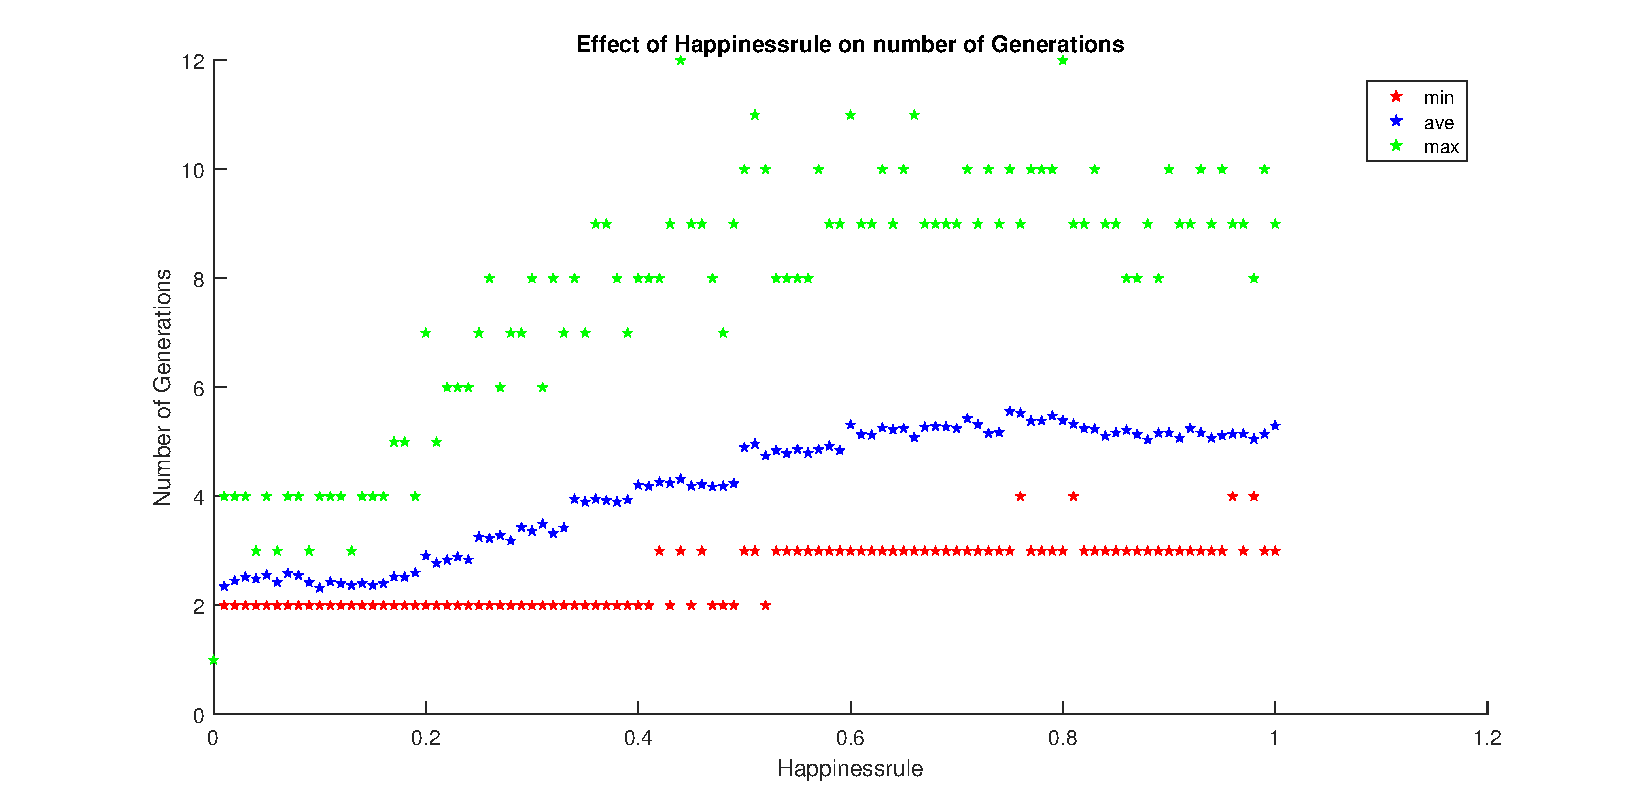
\includegraphics[width=0.9\textwidth]{happinessregel_aantgen_2.pdf}
    \caption{Influence of happiness rule on the number of generations until reaching the equilibrium. The green graph shows the maximum number of generations, the blue graph shows the average number of generations and the red graph shows the minimum number of generations}
    \label{fig:avegen}
\end{figure}
\\
It is also interesting to investigate how the random variable $Y_j$, which we denote as the number of generations it takes to reach the equilibrium under HR $j$, is distributed, and how the distribution is influenced by the HR. For that reason, we ran 10000 simulations for each HR(1/4,1/3,1/2 and 1) and plotted some histograms(figure\ref{fig:histogram}). We chose bin size 1 for each histogram because $Y_j$ is a random variable that only takes integer values. So a histogram of bin size like 0.5 will not give any extra information and a loss of lots of information will occur if bin size 2 is chosen. 
\\
 
\begin{figure}[H]
	
    \centering
    \begin{subfigure}{0.4\textwidth}
        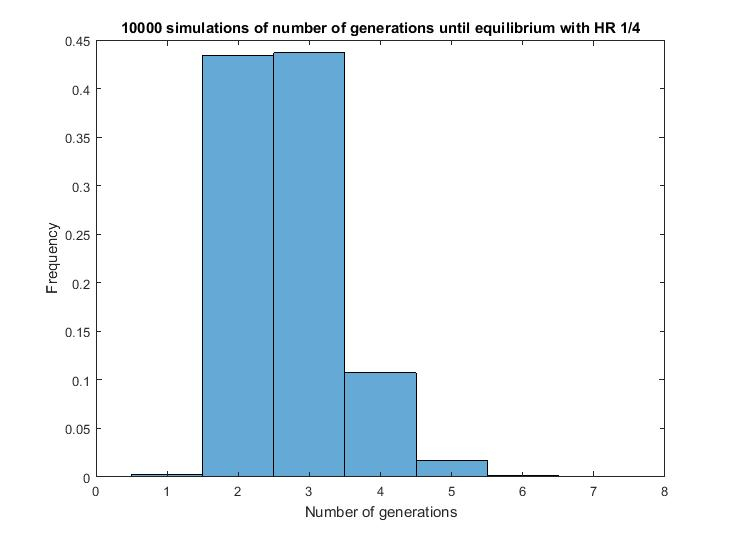
\includegraphics[width=\textwidth]{GenormHistogramAantalgen4}
        \caption{10000 simulations of number of generations until equilibrium with HR 1/4}
        \label{fig:gull}
    \end{subfigure}
    ~ %add desired spacing between images, e. g. ~, \quad, \qquad, \hfill etc. 
      %(or a blank line to force the subfigure onto a new line)
    \begin{subfigure}{0.4\textwidth}
        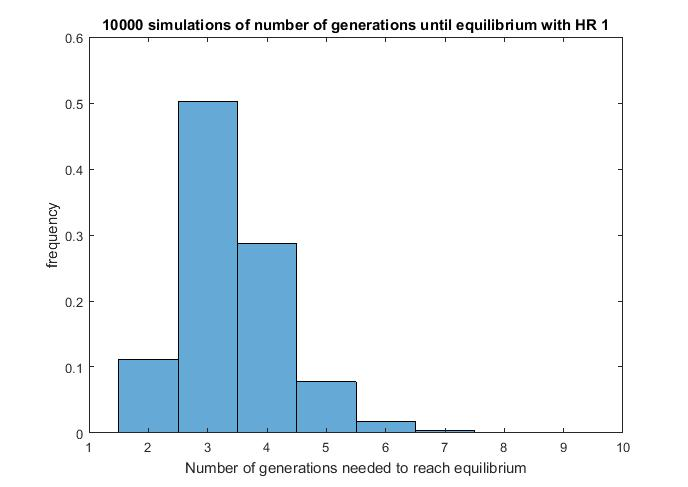
\includegraphics[width=\textwidth]{GenormHistogramAantalgen}
        \caption{10000 simulations of number of generations until equilibrium with HR 1/3}
        \label{fig:tiger}
    \end{subfigure}
    ~ %add desired spacing between images, e. g. ~, \quad, \qquad, \hfill etc. 
    %(or a blank line to force the subfigure onto a new line)
    \begin{subfigure}{0.4\textwidth}
        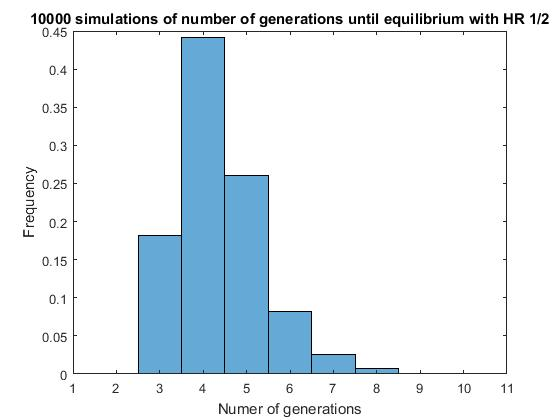
\includegraphics[width=\textwidth]{GenormHistogramAantalgen2}
        \caption{10000 simulations of number of generations until equilibrium with HR 1/2}
        \label{minimal happiness 1}
    \end{subfigure}
    \begin{subfigure}{0.4\textwidth}
        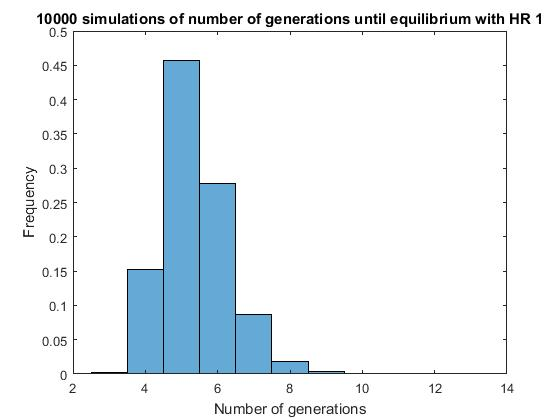
\includegraphics[width=\textwidth]{GenormHistogramAantalgen1}
        \caption{10000 simulations of number of generations until equilibrium with HR 1}
        \label{minimal happiness 2}
    \end{subfigure}
    \caption{The probability distribution of $Y$ (the number of generations until reaching the equilibrium) is approximated with a histogram of bin size 1. For each HR(1/4, 1/3, 1/2 and 1), 10000 simulations were ran.}\label{fig:histogram}
\end{figure}

Looking at the histograms, all $Y_j$'s ($j\in \{1/2,1/3,1/4,1\}$) might come from the same distribution, but with different parameters, since their sample means are obviously different.\\
In an attempt to find a good(confidence level 95\%) fit for the distribution of $Y_{1/3}$, we've used the chi-squared goodness of fit test(chi2gof) to see whether $Y_{1/3}$ is Poisson distributed. We first used the 'fitdist'-function of Matlab to calculate the maximal likelihood estimater for $\hat{\lambda}$ and then performed the chi-sqaured test. The test has rejected the null-hypothesis $H_0:Y_{1/3}\sim\text{Poisson}(\hat{\lambda})$ with significance level $\alpha=0.05$. \\   
\\
With the same method, we've also tested whether $Y_{1/3}$ is binomial or negative binomial distributed. But again, they have been rejected by the chi-sqaured test. So we can only conclude that $Y_{1/3}$ is not Poisson, binomial and negative binomial distributed.\\
\\
In order to make a better comparison of the distribution between $Y_{1/3},Y_{1/4},Y_{1/2}$ and $Y_1$, we made some QQ-plots, which is shown in figure \ref{fig:QQ-plot}.\\ 
\begin{figure}[H]
	
    \centering
    \begin{subfigure}{0.6\textwidth}
        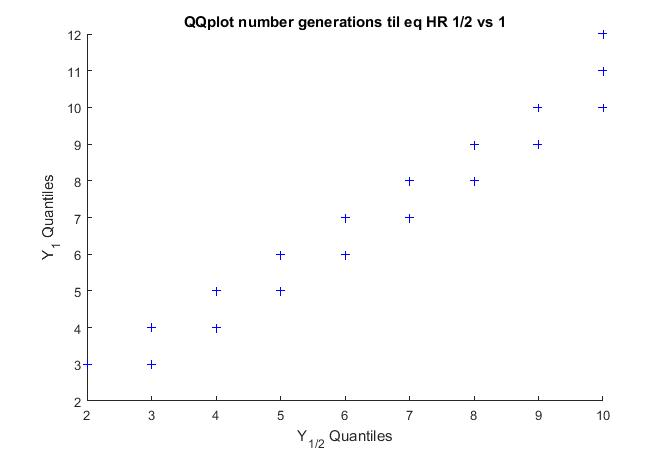
\includegraphics[width=\textwidth]{QQplotATGEN3}
        \caption{QQ-plot of $Y_{1}$ vs $Y_{1/2}$}
        \label{fig:QQplotATGEN3}
    \end{subfigure}
    ~ %add desired spacing between images, e. g. ~, \quad, \qquad, \hfill etc. 
      %(or a blank line to force the subfigure onto a new line)
    \begin{subfigure}{0.6\textwidth}
        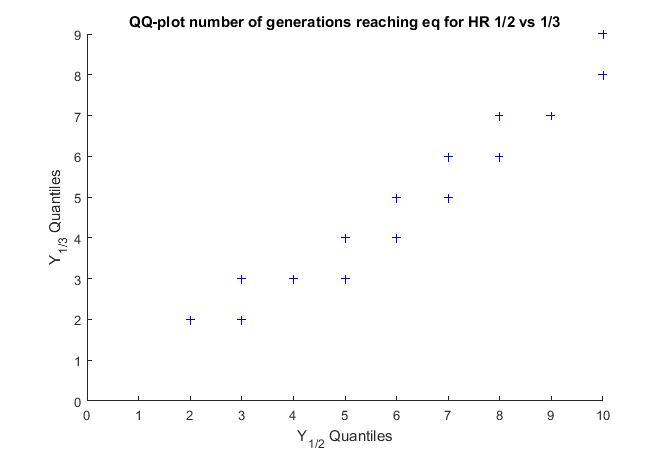
\includegraphics[width=\textwidth]{QQplotATGEN1}
        \caption{QQ-plot of $Y_{1/3}$ vs $Y_{1/2}$}
        \label{fig:QQplotATGEN1}
    \end{subfigure}
    \begin{subfigure}{0.6\textwidth}
        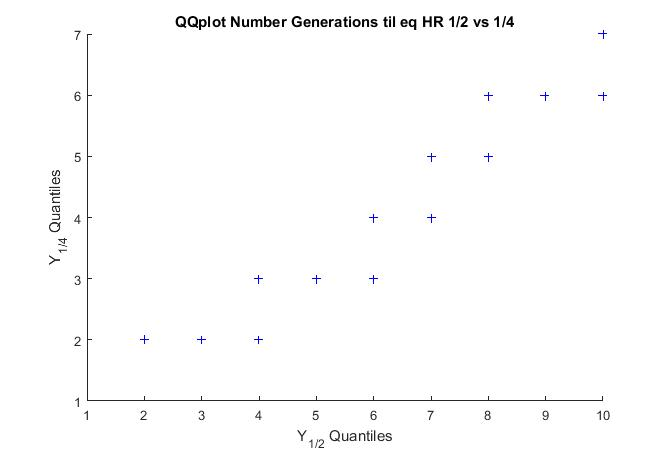
\includegraphics[width=\textwidth]{QQplotATGEN2}
        \caption{QQ-plot of $Y_{1/4}$ vs $Y_{1/2}$}
        \label{fig:QQplotATGEN2}
    \end{subfigure}
    \caption{QQ-plot of $Y_{1}$ vs $Y_{1/2}$, $Y_{1/3}$ vs $Y_{1/2}$ and $Y_{1/4}$ vs $Y_{1/2}$}\label{fig:QQ-plot}
\end{figure}
As expected, the QQ-plots have a stairwise pattern. This is because our data came from a discrete random variable. We see that the plots appears linear, especially the plot of $Y_{1}$ vs $Y_{1/2}$. The plot indicates that these 4 $Y_j$'s might belong to the location-scale family of some distribution.\\
\\
With the two-sample kolomogorov-smirnov test(kstest2) of significance level $\alpha=0.05$ in Matlab, which has null-hypothesis $H_0:F(X)=G(Y)$ for $F,G$ the CDF of $X$ and $Y$, it can be concluded that these $Y_j$'s don't come from the same distribution with the same parameters. Unfortunately, we weren't able to find a test that tests whether these $Y_j$'s comes from the same family distribution(i.e. same distribution but different parameter values).\\
\\
%Interesting to note though, is that both the mean and the variance increase with the happiness rule. In line with the following section, we see a relatively small mean and relatively often large number of generations.\\
%\textbf{Partial explanation.} While not immediately intuitive, the relatively small mean cannot be immediately explained. However we do have an explanation for the relatively high frequency for the large number of generations. If, after a few generations, we do not have equilibrium, moving to a better location gets harder. Further details are provided in the following section. Thus, reaching equilibrium eats relatively much time.